% !TeX program = lualatex
% !TeX encoding = utf-8
% !TeX spellcheck = ru_RU
%==========================================================
% v. 3.2
% Отчет может быть откомпилирован в LuaLaTeX.
% Например в дистирибутивах MikTeX или TeXlive
% (требуется установка пакета minted), а также
% в он-лайн версии https://www.overleaf.com/
% (включите компилятор LuaLaTeX).
%
% Для создания документа может потребоваться несколько
% запусков его компиляции. Например, обновление содержания
% требует двойной компиляции.
%
% Обратите внимание на команду команда сжатия/растяжения
% текста \textls из пакета microtype (см. пример).
%==========================================================
\documentclass[14pt]{extarticle}
\usepackage[main=russian,english]{babel} % языковая поддержка
\usepackage{amsmath, amssymb, unicode-math}% пакеты для набора математики
\usepackage[explicit]{titlesec} % настройка заголовков
\usepackage{titletoc} % настройка содержания
\usepackage{enumitem} % настройка нумерованных списков
\setlist{nosep, wide} % убрать вертикальные отступы, текст всю ширину
\usepackage{cite} % ссылки на литературу [1-10]
\usepackage[tracking=true]{microtype} % микротипографика
\microtypecontext{kerning=russian} % настройка микротипографики
\usepackage{geometry} % настройка геометрии страницы
\usepackage{graphicx} % поддержка графики
\usepackage{indentfirst} % красная строка в первом абзаце
\usepackage{float}
\usepackage{tabularx}
%========================================
\babelfont{rm}[Scale=0.976]{Times New Roman} % шрифт с засечками для кириллицы
% если нужен шрифт без засечек в документе, то подключаем его
%\babelfont{sf}[Scale=MatchLowercase]{Arial} % шрифт без засечек
% Scale=MatchLowercase - масштабировать выбранный шрифт в соответствии с
% текущим римским шрифтом по умолчанию до высоты строчных
\babelfont{tt}[Scale=0.976]{Courier New} % моноширинный шрифт
%========================================
\usepackage{xcolor} % поддержка цвета
\usepackage{hyperref} % гипертекстовые ссылоки в документе
\usepackage{verbatim} % используем из этого пакета окружение comment для многострочных комментариев
\usepackage{tabularray} % для создания таблиц
\usepackage{tikz} % пакет для рисования
\usetikzlibrary{calc, decorations.pathmorphing, shapes, arrows, chains, positioning, shapes.misc, fit} % библиотеки для пакета tikz

\tikzset{
	line/.style={draw, -latex'},
	every join/.style={line},
	u/.style={anchor=south},
	r/.style={anchor=west},
	fxd/.style={text width = 6em},
	it/.style={font={\small\itshape}},
	bf/.style={font={\small\bfseries}}
}
\tikzstyle{base} =
	[
		draw,
		on chain,
		on grid,
		align=center,
		minimum height=4ex,
		minimum width = 10ex,
		node distance = 6mm and 60mm,
		text badly centered
	]
\tikzstyle{coord} =
	[
		coordinate,
		on chain,
		on grid
	]
\tikzstyle{cloud} =
	[
		base,
		ellipse,
		node distance = 3cm,
		minimum height = 2em
	]
\tikzstyle{decision} =
	[
		base,
		diamond,
		aspect=2,
		node distance = 2cm,
		inner sep = 0pt
	]
\tikzstyle{block} =
	[
		rectangle,
		base,
		rounded corners,
		minimum height = 2em
	]
\tikzstyle{print_block} =
	[
		base,
		tape,
		tape bend top=none,
	]
\tikzstyle{io} =
	[
		base,
		trapezium,
		trapezium left angle = 70,
		trapezium right angle = 110,
	]
\makeatletter
\pgfkeys{/pgf/.cd,
	subrtshape w/.initial=2mm,
	cycleshape w/.initial=2mm
}
\pgfdeclareshape{subrtshape}{
	\inheritsavedanchors[from=rectangle]
	\inheritanchorborder[from=rectangle]
	\inheritanchor[from=rectangle]{north}
	\inheritanchor[from=rectangle]{center}
	\inheritanchor[from=rectangle]{west}
	\inheritanchor[from=rectangle]{east}
	\inheritanchor[from=rectangle]{mid}
	\inheritanchor[from=rectangle]{base}
	\inheritanchor[from=rectangle]{south}
	\backgroundpath{
		\southwest \pgf@xa=\pgf@x \pgf@ya=\pgf@y
		\northeast \pgf@xb=\pgf@x \pgf@yb=\pgf@y
		\pgfmathsetlength\pgfutil@tempdima{\pgfkeysvalueof{/pgf/subrtshape w}}
		\def\ppd@offset{\pgfpoint{\pgfutil@tempdima}{0ex}}
		\def\ppd@offsetm{\pgfpoint{-\pgfutil@tempdima}{0ex}}
		\pgfpathmoveto{\pgfqpoint{\pgf@xa}{\pgf@ya}}
		\pgfpathlineto{\pgfqpoint{\pgf@xb}{\pgf@ya}}
		\pgfpathlineto{\pgfqpoint{\pgf@xb}{\pgf@yb}}
		\pgfpathlineto{\pgfqpoint{\pgf@xa}{\pgf@yb}}
		\pgfpathclose
		\pgfpathmoveto{\pgfpointadd{\pgfpoint{\pgf@xa}{\pgf@yb}}{\ppd@offsetm}}
		\pgfpathlineto{\pgfpointadd{\pgfpoint{\pgf@xa}{\pgf@ya}}{\ppd@offsetm}}
		\pgfpathlineto{\pgfpointadd{\pgfpoint{\pgf@xb}{\pgf@ya}}{\ppd@offset}}
		\pgfpathlineto{\pgfpointadd{\pgfpoint{\pgf@xb}{\pgf@yb}}{\ppd@offset}}
		\pgfpathclose
	}
}
\pgfdeclareshape{cyclebegshape}{
	\inheritsavedanchors[from=rectangle]
	\inheritanchorborder[from=rectangle]
	\inheritanchor[from=rectangle]{north}
	\inheritanchor[from=rectangle]{center}
	\inheritanchor[from=rectangle]{west}
	\inheritanchor[from=rectangle]{east}
	\inheritanchor[from=rectangle]{mid}
	\inheritanchor[from=rectangle]{base}
	\inheritanchor[from=rectangle]{south}
	\backgroundpath{
		\southwest \pgf@xa=\pgf@x \pgf@ya=\pgf@y
		\northeast \pgf@xb=\pgf@x \pgf@yb=\pgf@y
		\pgfmathsetlength\pgfutil@tempdima{\pgfkeysvalueof{/pgf/cycleshape w}}
		\pgfpathmoveto{\pgfqpoint{\pgf@xa}{\pgf@ya}}
\pgfpathlineto{\pgfpointadd{\pgfpoint{\pgf@xa}{\pgf@yb}}{\pgfpoint{0ex}{-\pgfutil@tempdima}}}
\pgfpathlineto{\pgfpointadd{\pgfpoint{\pgf@xa}{\pgf@yb}}{\pgfpoint{\pgfutil@tempdima}{0ex}}}
\pgfpathlineto{\pgfpointadd{\pgfpoint{\pgf@xb}{\pgf@yb}}{\pgfpoint{-\pgfutil@tempdima}{0ex}}}
\pgfpathlineto{\pgfpointadd{\pgfpoint{\pgf@xb}{\pgf@yb}}{\pgfpoint{0ex}{-\pgfutil@tempdima}}}
\pgfpathlineto{\pgfqpoint{\pgf@xb}{\pgf@ya}}
		\pgfpathclose
	}
}
\pgfdeclareshape{cycleendshape}{
	\inheritsavedanchors[from=rectangle]
	\inheritanchorborder[from=rectangle]
	\inheritanchor[from=rectangle]{north}
	\inheritanchor[from=rectangle]{center}
	\inheritanchor[from=rectangle]{west}
	\inheritanchor[from=rectangle]{east}
	\inheritanchor[from=rectangle]{mid}
	\inheritanchor[from=rectangle]{base}
	\inheritanchor[from=rectangle]{south}
	\backgroundpath{
		\southwest \pgf@xa=\pgf@x \pgf@ya=\pgf@y
		\northeast \pgf@xb=\pgf@x \pgf@yb=\pgf@y
		\pgfmathsetlength\pgfutil@tempdima{\pgfkeysvalueof{/pgf/cycleshape w}}
		\pgfpathmoveto{\pgfqpoint{\pgf@xb}{\pgf@yb}}
\pgfpathlineto{\pgfpointadd{\pgfpoint{\pgf@xb}{\pgf@ya}}{\pgfpoint{0ex}{\pgfutil@tempdima}}}
\pgfpathlineto{\pgfpointadd{\pgfpoint{\pgf@xb}{\pgf@ya}}{\pgfpoint{-\pgfutil@tempdima}{0ex}}}
\pgfpathlineto{\pgfpointadd{\pgfpoint{\pgf@xa}{\pgf@ya}}{\pgfpoint{\pgfutil@tempdima}{0ex}}}
\pgfpathlineto{\pgfpointadd{\pgfpoint{\pgf@xa}{\pgf@ya}}{\pgfpoint{0ex}{\pgfutil@tempdima}}}
\pgfpathlineto{\pgfqpoint{\pgf@xa}{\pgf@yb}}
		\pgfpathclose
	}
}
\makeatother
\tikzstyle{subroutine} =
	[
		base,
		subrtshape,
	]
\tikzstyle{cyclebegin} =
	[
		base,
		cyclebegshape,
	]
\tikzstyle{cycleend} =
	[
		base,
		cycleendshape,
	]
\tikzstyle{connector} =
	[
		base,
		circle,
	]

\usepackage[open, numbered]{bookmark} % закладки в pdf с нумерацией
\usepackage{fancyhdr} % настройка колонтитулов страницы
\usepackage{setspace} % определение интервала в тексте
\usepackage[singlelinecheck=false]{caption} % настройка заголовков
\usepackage[newfloat]{minted} % листинги
\usepackage{csquotes} % расширенная языковая поддержка
%========================================
\renewcommand{\UrlFont}{\ttfamily\small} % определене размера шрифта small для ссылок url
%========================================
\setlength{\parindent}{1.25cm} % Отступ красной строки
% Для отступов внутри заголовков глав, разделов и др. так как
% в них отступ может быть равен "0"
\newlength{\normalparindent} 
\setlength{\normalparindent}{\parindent}
%
\geometry{ % настройка страницы, шрифтов и отступов
	a4paper,
	left=25mm,
	right=10mm,
	top=20mm,
	bottom=20mm,
	headsep=5mm,
%	showframe % показать поля страниц
}
%========================================
% подавление висячих строк в тексте
\clubpenalty=10000
\widowpenalty=10000
%========================================
\spacing{
	0.976 % одинарный интервал
%	1.464 % полуторный интервал
}
%========================================
% настройка колонтитулов страницы
\pagestyle{fancy}
\fancyhf{} % очистка текущих значений
\setlength{\headheight}{0pt}
\fancyfoot[C]{\thepage} % номер страницы вверху по центру
\renewcommand{\headrule}{} % отключить линию в вверхнем колонтитуле
\fancypagestyle{plain}{ % номер страницы в центре для 1-й страницы chapter
	\fancyfoot[C]{\thepage}
}
%========================================
% настройка оформления списков
\setlist{nosep, wide} % убрать вертикальные отступы, текст всю ширину
%==========================================================
% настройка заголовков у рисунков, таблиц и листингов
\DeclareCaptionLabelSeparator{defffis}{~--~}
\captionsetup[table]{aboveskip=6pt plus 3pt minus 3pt, belowskip=6pt plus 3pt minus 3pt, margin={\normalparindent, 0pt}, indention=-\normalparindent, labelsep=defffis, font=normalsize}
\captionsetup[figure]{aboveskip=6pt plus 3pt minus 3pt, belowskip=6pt plus 3pt minus 3pt, justification=centering, labelsep=defffis, font=normalsize}
\captionsetup[listing]{aboveskip=-14pt plus 3pt minus 3pt, belowskip=6pt plus 3pt minus 3pt, margin={\normalparindent, 0pt}, indention=-\normalparindent, labelsep=defffis, font=normalsize}
% настройка заголовков для многостраничных таблиц longtblr пакет tabularray
\DefTblrTemplate{firsthead}{default}{\addtocounter{table}{-1}\captionof{table}[\InsertTblrText{entry}]{\InsertTblrText{caption}}}
\DefTblrTemplate{middlehead,lasthead}{default}{\addtocounter{table}{-1}\captionof{table}[]{\InsertTblrText{caption}~(Продолжение)}}
\DefTblrTemplate{contfoot-text}{default}{\centerline{Продолжение на следующей странице}}
\SetTblrTemplate{caption-lot}{empty}
%==========================================================
% настройка визуализации листингов
% https://pygments.org/demo/#try - тут можно попробовать разные стили
\setminted{xleftmargin=0.5cm, linenos, numbersep=5pt, breaklines, breakanywhere, frame=single, framesep=1ex,  fontsize=\small} % настройки оформления листингов
% создание окружения code для оформления
% многостраничных листингов
\newenvironment{code}{\captionsetup{type=listing, belowskip=-14pt plus 3pt minus 0pt}}{}
\SetupFloatingEnvironment{listing}{name=сode}
\AtBeginEnvironment{code}{\vspace{28pt plus 3pt minus 0pt}} % добавляем отступ перед окружением code
% команда удалемния пробела после окружения
\newcommand{\nospacebetweenenvs}{%
	\vspace{-\glueexpr(\topsep+\partopsep)*2}%
}
% настройка отсупов после окружения listing
\AtEndEnvironment{listing}{\nospacebetweenenvs\vspace{12pt plus 3pt minus 0pt}}
%==========================================================
% определяем стандартные названия
\addto\captionsrussian{\def\figurename{Рис.}} % подпись для рисунка
\addto\captionsrussian{\def\tablename{Табл.}} % подпись для таблицы
\addto\captionsrussian{\def\listingname{Лист.}} % подпись для листинга
%==========================================================
\makeatletter
\newcommand{\hrf}[1]{\hbox to #1{\hrulefill}} % команда подчеркивания
%==========================================================
% настройка заголовков и их отоборажения в содержании
\renewcommand{\@pnumwidth}{1.25em} % настройка отступа под номер страницы в содержании
% настройка оформления в тексте и содержании для section
\titleformat{\section}[block]
{\hspace*{\normalparindent}\normalfont\bfseries}
{\thesection}
{1ex}
{#1}
[]
%
\titlespacing*{\section}{0pt}{14pt plus 2pt minus 2pt}{14pt plus 2pt minus 2pt}
%
\titlecontents{section}
[0pt]
{}
%{\makebox[1.25em][l]{\thecontentslabel}} % второй вариант оформления
{\contentspush{\makebox[1.25em][l]{\thecontentslabel}}} % второй вариант оформления: добавляет отступ под номер для всех строк заголовка в содержании (смотреть на многострочных заголовках)
{}
{\nolinebreak\titlerule*[1pc]{.}\contentspage} % \nolinebreak добавлен для предотвращения нежелательных разрывов строк между заголовками и номерами страниц
[]
%==========================================================
% создание нового вида секции в документе
\newcounter{sectionc} % создание счетчика для sectionc
\titleclass{\sectionc}{straight}[\part] % создание новой секции sectionc
% секция sectionc является подчиненной \part
% для класса article ToC level(part)=0, тогда ToC level(sectionc)=1
% т.е. ToC level(section)=ToC level(sectionc)
% straight - означает, что секция может быть использовна
% в любом месте страницы
% настройка оформления в тексте и содержании для sectionс
\titleformat{\sectionc}[block]
{\normalfont\bfseries}
{}
{0pt}
{\filcenter #1}
[]
%
\titlespacing*{\sectionc}{0pt}{14pt plus 2pt minus 2pt}{14pt plus 2pt minus 2pt}
%
\titlecontents{sectionc}
[0em]
{\normalfont}
{}
{}
{\nolinebreak\titlerule*[1pc]{.}\contentspage}
[]
%==========================================================
% для корректного вывода закладок в PDF при просмотре
\def\toclevel@sectionc{1} % настройка уровня нового вида секций
% команды для вкл/откл номера в закладках
\newcommand{\numbersections}{\renewcommand{\Hy@numberline}[1]{##1~}}
\newcommand{\nonumbersections}{\renewcommand{\Hy@numberline}[1]{}}
% включаем нумерацию для section переопределяя команду
\let\oldsection\section
\renewcommand{\section}{\numbersections\oldsection}
% отключаем нумерацию для sectionc переопределяя команду
\let\oldsectionc\sectionc
\renewcommand{\sectionc}{\nonumbersections\oldsectionc}
%==========================================================
% содержание по центру
\renewcommand\tableofcontents{
	\pdfbookmark[sectionc]{\contentsname}{toc} % Добавляем Содержание в закладку PDF ToC
	\sectionc*{\contentsname
		\@mkboth{\contentsname}{\contentsname}}
	\@starttoc{toc}
}
%==========================================================
% настройка списка литературы
\renewenvironment{thebibliography}[1]{
	\sectionc{Список использованных источников}
	\@mkboth{\MakeUppercase\refname}{\MakeUppercase\refname}%
	\begin{enumerate}[label=\arabic*., fullwidth, nosep, itemindent=\parindent, 
		listparindent=\parindent]
		\@openbib@code
		\sloppy
		\clubpenalty4000
		\@clubpenalty \clubpenalty
		\widowpenalty4000
		\sfcode`\.\@m}
	{\def\@noitemerr
		{\@latex@warning{Empty `thebibliography' environment}}%
\end{enumerate}}

\newcounter{oldtocdepth}

\newcommand{\hidefromtoc}{%
  \setcounter{oldtocdepth}{\value{tocdepth}}%
  \addtocontents{toc}{\protect\setcounter{tocdepth}{-10}}%
}

\newcommand{\unhidefromtoc}{%
  \addtocontents{toc}{\protect\setcounter{tocdepth}{\value{oldtocdepth}}}%
}

%==========================================================
\makeatother
\graphicspath{{pic/}} % папка с рисунками
\begin{document}
%%%%%%%%%%%%%%%%%%%%%%%%%%%%%%%%%%%%
%                                  %
%          Титульный лист          %
%                                  %
%%%%%%%%%%%%%%%%%%%%%%%%%%%%%%%%%%%%
% Выравнивание контента по центру можно делать разными способами
% \centerline{...} - выравнивает строку по центру (для одной строки!)
% \begin{center} - окружение для выравнивания по центру (добавлят вертикальный отступы до и после)
%  ...
% \end{center}
% {\par\centering - окружение для выравнивания по центру без добавления вертикальных отступов
% ...
% \par}
{\par\centering % окружение для выравнивания по центру


\includegraphics[width=0.12\linewidth]{logo.pdf} % вставляем логотип

МИНИСТЕРСТВО ЦИФРОВОГО РАЗВИТИЯ, СВЯЗИ И\\МАССОВЫХ КОММУНИКАЦИЙ РОССИЙСКОЙ ФЕДЕРАЦИИ\\[5mm] % новый абзац + отступ 5мм
% \textbf - делает шрифт жирным

Ордена Трудового Красного Знамени федеральное государственное\\ бюджетное образовательное учреждение высшего образования\\ «\textbf{Московский технический университет связи и информатики}»\\(\textbf{МТУСИ})\\[5mm] 
	
Кафедра «Сетевые информационные технологии и сервисы»
\par}

\begin{tikzpicture}[overlay, remember picture] % рисуем рамку на титульнике
	\draw[line width=0.5mm] 
	($(current page.north west) + (20mm, -10mm)$)
	rectangle
	($(current page.south east) + (-10mm, 10mm)$);
\end{tikzpicture}

\vfill\vfill % двойно бесконечный вертикальный промежуток (работает как пружина)

{\par\centering
\textbf{ОТЧЕТ}\\ по лабораторной работе №\,2\\[5mm]

по дисциплине «\textbf{Сетевые технологии}»
\par}

\vfill % бесконечный вертикальный промежуток

\hfill % бесконечный горизонтальный промежуток (работает как пружина)
\begin{minipage}{0.45\textwidth} % министраница шириной 0.45 от ширины текста
	Выполнил:\\[2mm]
	студент гр.\,БФИ2202\\[2mm]
	\hrf{2.7cm}\,Сидорук Д.\,В.\\[2mm]
	«\,\hrf{1cm}\,»\,\hrf{2.5cm}\,\the\year{}\,г.\\[5mm]
	
	Проверил:\\[2mm]
	к.т.н., доцент\\[2mm]
	\hrf{2.7cm}\,Галицкий М.\,В.\\[2mm]
	«\,\hrf{1cm}\,»\,\hrf{2.5cm}\,\the\year{}\,г.
\end{minipage}%

\vfill

\centerline{Москва, \the\year{}\,г.} % строка по центру
\thispagestyle{empty} % стиль страницы отсутствует (без номера страницы)
%%%%%%%%%%%%%%%%%%%%%%%%%%%%%%%%%%%%
%                                  %
%            Содержание            %
%                                  %
%%%%%%%%%%%%%%%%%%%%%%%%%%%%%%%%%%%%
\newpage % новая страницы
\tableofcontents % содержание
%%%%%%%%%%%%%%%%%%%%%%%%%%%%%%%%%%%%
%                                  %
%         Тело документа           %
%                                  %
%%%%%%%%%%%%%%%%%%%%%%%%%%%%%%%%%%%%
\newpage % новая страница

\section{Цель работы}

Изучить принципы построения простейших сетей и их настройки с использованием симулятора компьютерных сетей.

Собрать в соответствии с заданной топологией сеть, запустить и настроить виртуальное оборудование.

\section{Задание}

\begin{enumerate}
    \item Организовать простейшие сети: компьютер-коммутатор-маршрутизатор-коммутатор-компьютер.
    \item Запустить и настроить виртуальное оборудование.
    \item Изучить полученную информацию и оформить ее в соответствии с требованиями.
\end{enumerate}

\section{Ход работы}

На рисунке ниже представлен общий вид построенной сети. (\ref{img:ОбщийВид})

\begin{figure}[H]
    \centering
    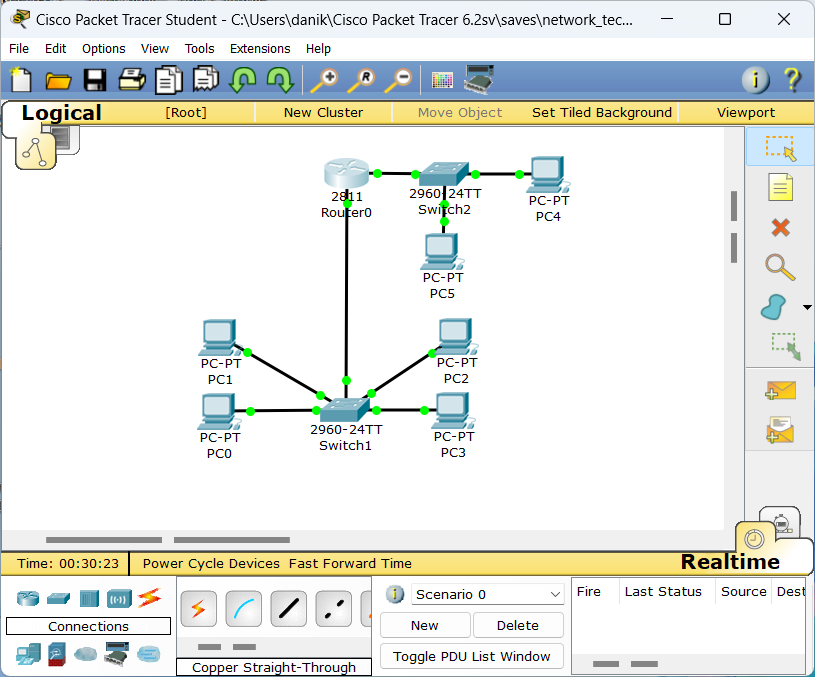
\includegraphics[width=1.0\linewidth]{ОбщийВид.png}
    \caption{Общий вид построенной сети\label{img:ОбщийВид}}
\end{figure}

На рисунке ниже представлены настройки IP для PC0. (\ref{img:PC0})

\begin{figure}[H]
    \centering
    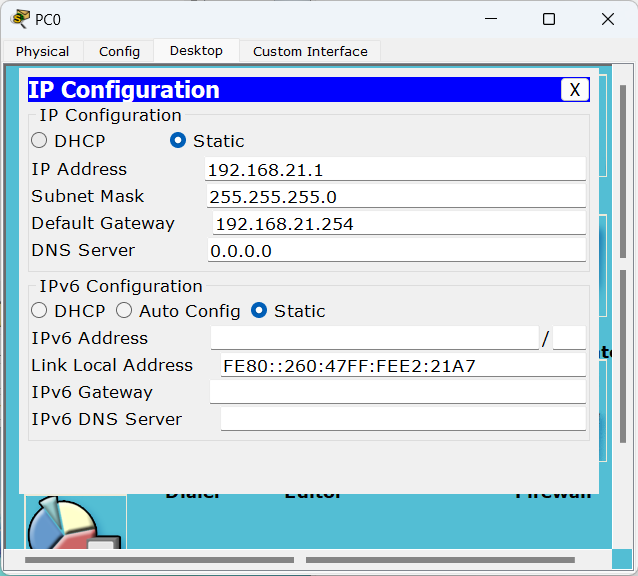
\includegraphics[width=1.0\linewidth]{PC0.png}
    \caption{Настройки IP для PC0\label{img:PC0}}
\end{figure}

На рисунке ниже представлены настройки IP для PC1. (\ref{img:PC1})

\begin{figure}[H]
    \centering
    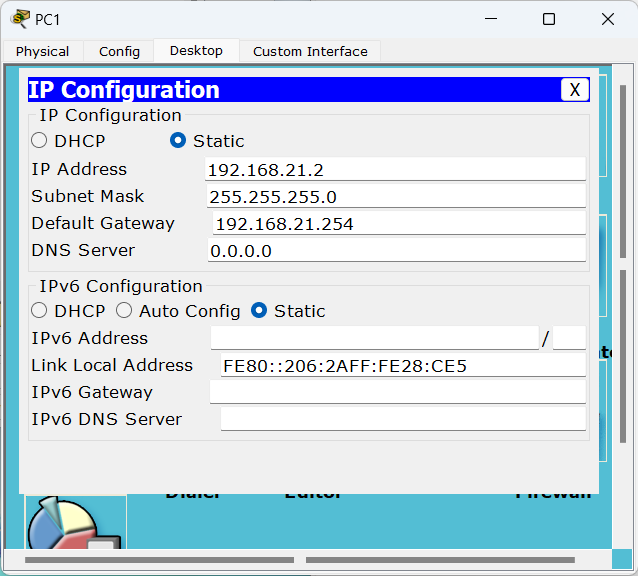
\includegraphics[width=1.0\linewidth]{PC1.png}
    \caption{Настройки IP для PC1\label{img:PC1}}
\end{figure}

На рисунке ниже представлены настройки IP для PC2. (\ref{img:PC2})

\begin{figure}[H]
    \centering
    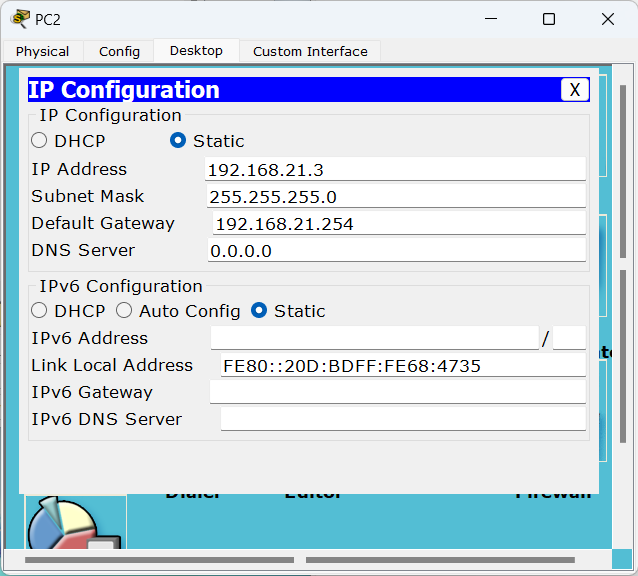
\includegraphics[width=1.0\linewidth]{PC2.png}
    \caption{Настройки IP для PC2\label{img:PC2}}
\end{figure}

На рисунке ниже представлены настройки IP для PC3. (\ref{img:PC3})

\begin{figure}[H]
    \centering
    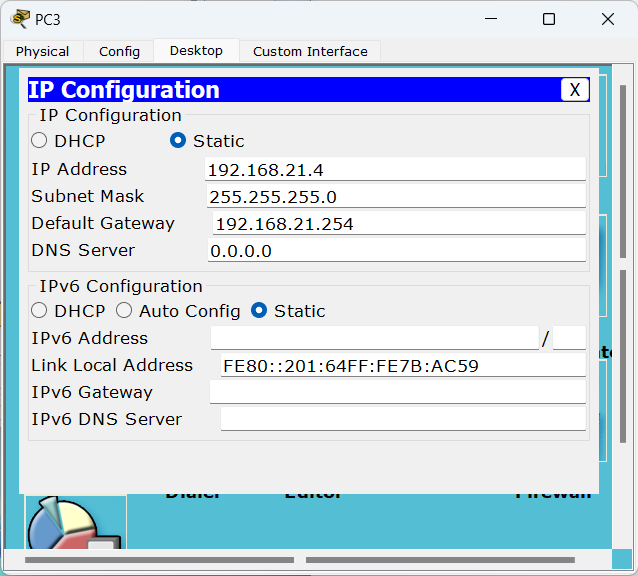
\includegraphics[width=1.0\linewidth]{PC3.png}
    \caption{Настройки IP для PC3\label{img:PC3}}
\end{figure}

На рисунке ниже представлены настройки IP для PC4. (\ref{img:PC4})

\begin{figure}[H]
    \centering
    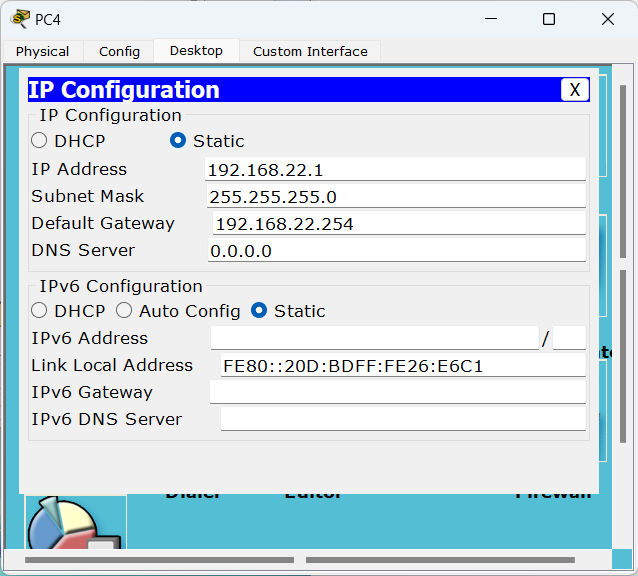
\includegraphics[width=1.0\linewidth]{PC4.png}
    \caption{Настройки IP для PC4\label{img:PC4}}
\end{figure}

На рисунке ниже представлены настройки IP для PC5. (\ref{img:PC5})

\begin{figure}[H]
    \centering
    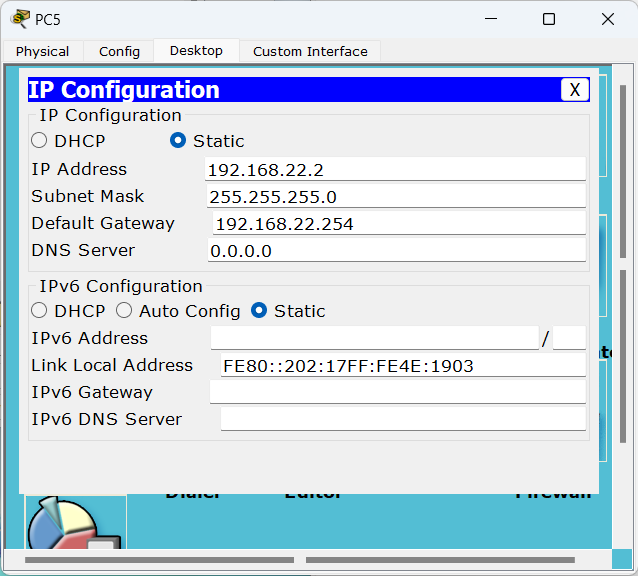
\includegraphics[width=1.0\linewidth]{PC5.png}
    \caption{Настройки IP для PC5\label{img:PC5}}
\end{figure}

На рисунке ниже представлены настройки интерфейса FastEthernet0/0 для Router0. (\ref{img:Router0FastEthernet0})

\begin{figure}[H]
    \centering
    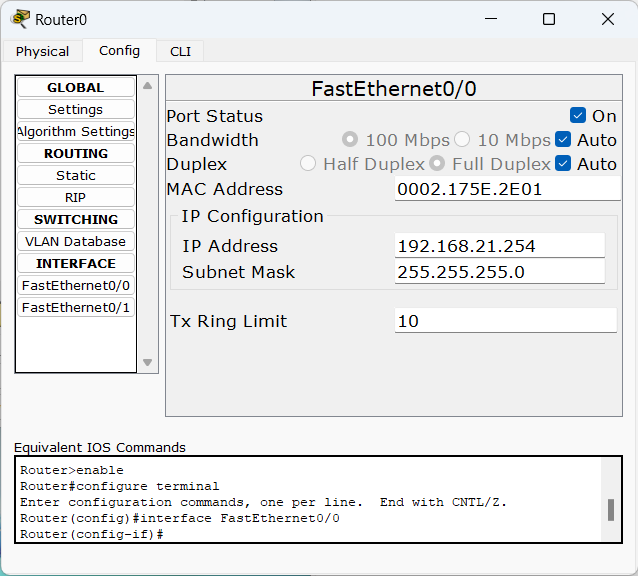
\includegraphics[width=1.0\linewidth]{Router0FastEthernet0.png}
    \caption{Настройки интерфейса FastEthernet0/0 для Router0\label{img:Router0FastEthernet0}}
\end{figure}

На рисунке ниже представлены настройки интерфейса FastEthernet0/1 для Router0. (\ref{img:Router0FastEthernet1})

\begin{figure}[H]
    \centering
    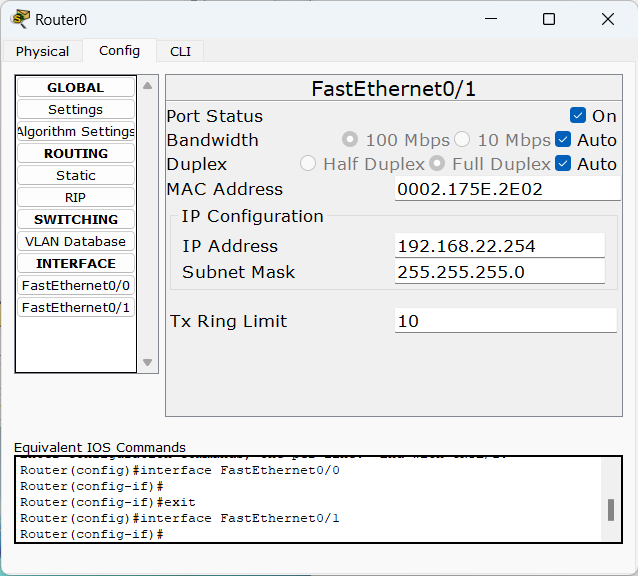
\includegraphics[width=1.0\linewidth]{Router0FastEthernet1.png}
    \caption{Настройки интерфейса FastEthernet0/1 для Router0\label{img:Router0FastEthernet1}}
\end{figure}

На рисунке ниже представлен результат выполнения команды \mintinline{bash}{ping 192.168.21.2} на PC0. (\ref{img:PC0Ping1})

\begin{figure}[H]
    \centering
    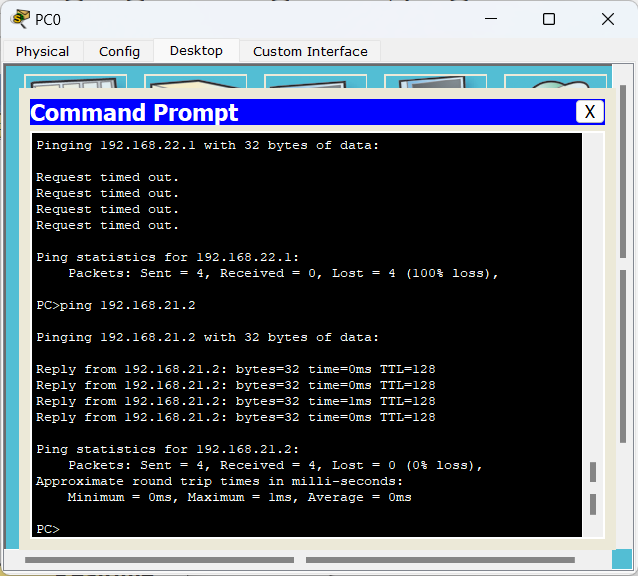
\includegraphics[width=1.0\linewidth]{PC0Ping1.png}
    \caption{Результат выполнения команды ping на PC0\label{img:PC0Ping1}}
\end{figure}

На рисунке ниже представлен результат выполнения команды \mintinline{bash}{ping 192.168.22.1} на PC0. (\ref{img:PC0Ping4})

\begin{figure}[H]
    \centering
    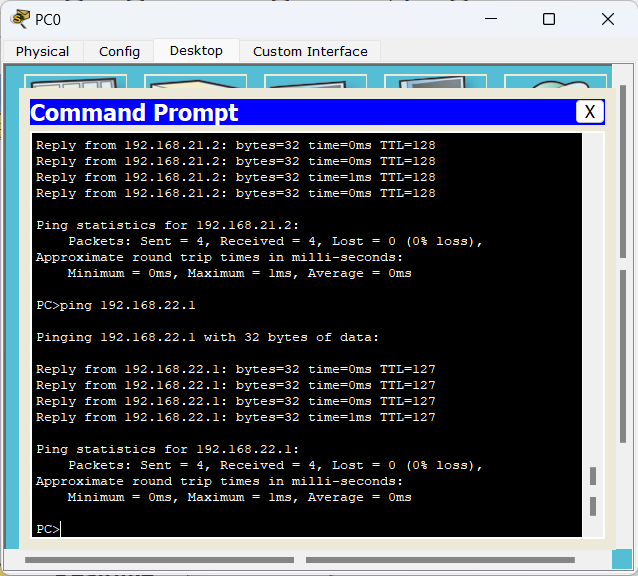
\includegraphics[width=1.0\linewidth]{PC0Ping4.png}
    \caption{Результат выполнения команды ping на PC0\label{img:PC0Ping4}}
\end{figure}

На рисунке ниже представлен результат выполнения команды \mintinline{bash}{ping 192.168.22.2} на PC4. (\ref{img:PC4Ping5})

\begin{figure}[H]
    \centering
    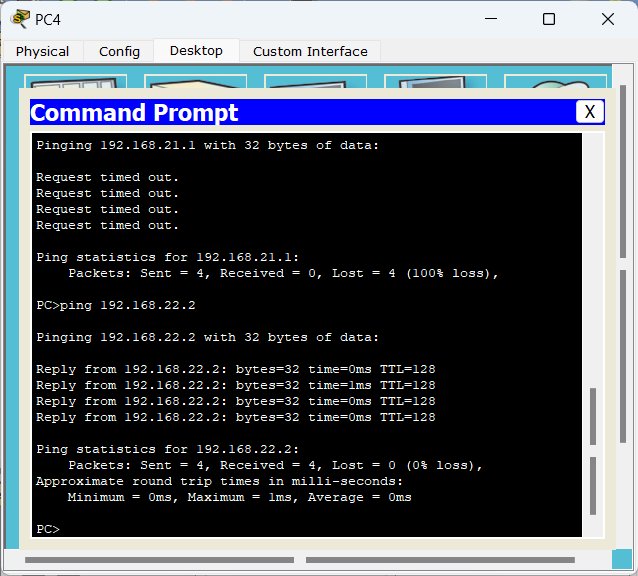
\includegraphics[width=1.0\linewidth]{PC4Ping5.png}
    \caption{Результат выполнения команды ping на PC4\label{img:PC4Ping5}}
\end{figure}

На рисунке ниже представлен результат выполнения команды \mintinline{bash}{ping 192.168.21.1} на PC4. (\ref{img:PC4Ping0})

\begin{figure}[H]
    \centering
    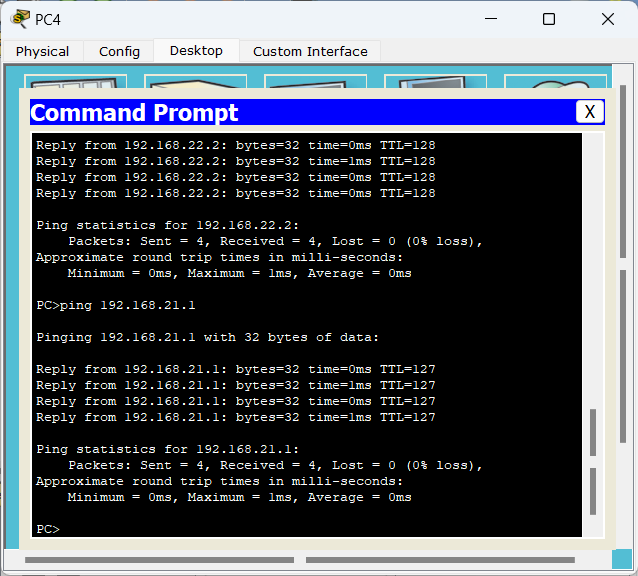
\includegraphics[width=1.0\linewidth]{PC4Ping0.png}
    \caption{Результат выполнения команды ping на PC4\label{img:PC4Ping0}}
\end{figure}

Таким образом, сети, соединяющие PC0, PC1, PC2, PC3 и PC4, PC5 были успешно соединены.

\section{Контрольные вопросы}

\begin{enumerate}
    \item Вопрос: Какие типовые топологии сетей вам известны?

    Ответ: Мне известны \textbf{полносвязная топология}: в которой каждый компьютер непосредственно связан со всеми остальными; \textbf{ячеистая топология}, получаемая из полносвязной путем удаления некоторых связей; \textbf{кольцевая топология}, в которой данные передаются по кольцу от одного компьютера к другому; \textbf{звездообразная топология}, в которой каждый компьютер подключается непосредственно к общему центарльному устройству; \textbf{дерево}, представляющее собой сеть с использованием нескольких концентраторов, иерархически соединенных между собой звездообразными связями; \textbf{общая шина}, являющаяся частным случаем звезды, в которой в качестве центрального элемента выступает пассивный кабель.
    \item Вопрос: Каковы достоинства и недостатки известных типовых топологий сетей?

    Ответ: \textbf{полносвязная топология} требует слишком большое количество кабеля и портов в каждом из компьютеров; \textbf{кольцевая топология} является неустойчивой: в случае выхода из строя или отключения какого-либо компьютера связность всей сети окажется под угрозой; \textbf{звездообразная топология} требует приобретения специализированного оборудования и наращивание количества узлов в ней ограничено количеством портов в концентраторе; \textbf{общая шина} так же, как и \textbf{кольцевая топология}, является неустойчивой, так как любой дефект кабеля нарушит связность всей сети, и, кроме того, страдает низкой производительностью: в каждый момент времени только один компьютер может пропускать данные по сети.
    \item Вопрос: Опишите принцип действия сетевого концентратора (хаба)

    Ответ: Концентратор имеет множество равноправных портов, к которым с помощью витой пары, коаксиального кабеля или оптоволкна подключаются устройства Ethernet. Получив сигнал от одного из подключенных к нему устройств, концентратор транслирует его на все свои активные порты.
    \item Вопрос: Опишите принцип действия сетевого моста

    Ответ: Сетевой мост предназначен для объединение подсетей компьютерной сети в единую сеть; при получении из сети пакета мост определяет, принадлежит ли он данной подсети и, если принадлежит, передает пакет дальше в тот сегмент, которому он предназначен.
    \item Вопрос: Опишите принцип действия коммутатора

    Ответ: перед началом работы коммутатор создает таблицу коммутации, запоминая, какой MAC-адрес относится к какому из портов запоминая, к какому из портов относится какой хост с каким MAC-адресом. В дальнейшем, если на один из портов поступит кадр для определенного MAC, который ассоциируется с одним из портов, коммутатор перешлет кадр на данный порт. Если же MAC адрес получателя не ассоциирован с каким-либо из портов, то кадр будет отправлен на все порты, за исключением того порта, с которого он был получен и коммутатор в дальнейшем запомнит, с каким хостом ассоциирован данный кадр, благодаря тому, что правильный получатель отвечает коммутатору.
    \item Вопрос: Опишите принцип действия маршрутизатора

    Ответ: Маршрутизатор маршрутизирует трафик сети: определяет маршрут перемещения пакета с помощью таблицы маршрутизации; проверяет корректность пакета, определяет адрес его получателя и отправляет его по назначению с учетом очередности, фрагментации, фильтрации и других заданных параметров.
    \item Вопрос: В чем отличие между коммутатором и маршрутизатором?

    Ответ: Коммутатор работает на канальном уровне, маршрутизатор же работает на сетевом, в связи с чем может реализовывать более интеллектуальную маршрутизацию; коммутатор объединяет отдельные компьютерные узлы в единую сеть, тогда как маршрутизатор соединяет отдельные сети 
    \item Вопрос: Какие формы маршрутизации вам известны?

    Ответ: Мне известны \textbf{жесткая маршрутизация}, в которой адреса определяют точный маршрут дейтаграммы и путь от одного адреса к другому в которой может включать только одну сеть; и \textbf{свободная маршрутизация}, позволяющая пересылать дейтаграмму более чем через одну сеть.
    \item Вопрос: Что такое IP-адрес, какие функции он выполняет? Из каких частей состоит? Какие классы IP-адресов вы знаете?

    Ответ: IP-адрес представляет собой уникальную четырехбайтовую величину, выраженную в десятичных числах, разделенных точками в форме X.W.Y.Z, где точки используются для отделения байтов, и состояющую из двух частей: адреса сети и адреса хоста, идентифицирующего рабочую станцию в сетевом сегменте. IP адрес является уникальным числовым идентификатором хоста в компьютерной сети. Существует пять классов IP-адресов: A, B, C, D, E.
    \item Вопрос: Что такое подсеть и для чего она создаётся?

    Ответ: Подсеть — это подмножество сети или фрагменты сети, которые не пересекаются с другими подсетями. Подсети используется для разделения сети на сегменты с целью более эффективного использования доступных адресов.
    \item Вопрос: Что такое маска подсети? Какие функции она выполняет?

    Ответ: Маска подсети — это битовая 4-байтная маска, позволяющая разделить IP-адрес на адрес подсети и адрес хоста внутри этой подсети.
    \item Вопрос: Что такое команда ping? Зачем она нужна?

    Ответ: Команда ping посылает трассировочные пакеты по указанному IP адресу и замеряет время, за которое был получен на них ответ. Она позволяет проверять состояние удаленных хостов, находить и локализировать неподалки в программном и аппаратном обеспечении, обеспечивающем работу сетей, и тестировать их качество.
\end{enumerate}

\sectionc{Заключение}

Собрать в соответствии с заданной топологией сеть, запустить и настроить виртуальное оборудование.

В ходе выполнения данной работы были изучены принципы построения простейших сетей и их настройки с использованием симулятора компьютерных сетей. Было запущено и настроено виртуальное оборудование в собранной в соответствии с заданной топологией сети.

\end{document}